\documentclass[aspectratio=169,handout]{beamer}
\usepackage{pgfpages}
\setbeameroption{show notes}
\setbeameroption{show notes on second screen=right}
\usetheme[progressbar=frametitle]{metropolis}

\usepackage[english,german]{babel}
\usepackage[autostyle=true,german=quotes]{csquotes}

%Tikz
\usepackage{tikz}
\usetikzlibrary{arrows,shapes,positioning,shadows,trees,calc}

%Tables
\usepackage{longtable,booktabs}
\usepackage{tabularx}
\usepackage{ltablex}
\usepackage{paralist}

%listings
\usepackage{listings}


\title{Projekt Java Compiler}
\subtitle{Spezielle Kapitel der Praktischen Informatik: Compilerbau}
\author{Florian Engel, Robin Heinz, Pavel Karasik, Steffen Lindner, Arwed Mett}
\institute{Universität Tübingen}
\date{05.02.2018}

\begin{document}

	%Titlepage
	\begin{frame}
		\titlepage
	\end{frame}

	%Agenda
	\begin{frame}
		\frametitle{Agenda}
		\tableofcontents
	\end{frame}

	%Chapters
	\begin{frame}
	\frametitle{Allgemein}
	
\textbf{Aufgabenstellung:}

Entwickeln eines Mini-Java Compilers mit den zugehörigen Schritten: Lexer, Parser, TypChecker und Codegenerierung.
\end{frame}

\begin{frame}[fragile]
\frametitle{Allgemein: Ziel}

\textbf{Ziel} 

Korrektes Übersetzen der folgenden Klasse:

\begin{lstlisting}[language=Java]
class Fibonacci {
  int getFib(int n) {
    return (n < 2) ? n : getFib(n-1) + getFib(n-2);
  }
}
\end{lstlisting}	
\end{frame}



\begin{frame}{Featureliste}

Umgesetze Features (Auszug):

\begin{itemize}
	\item Ternary Operator
	\item For / While / DoWhile 
	\item If / If-Else / Switch-Case
	\item Pre- bzw. Post Inkrement/Dekrement
	\item Arithmetische Operatoren (+, -, /, div, mod, *) inklusive Zuweisung (+=, etc.)
\end{itemize}	
\end{frame}

\begin{frame}{Entwicklung}

Code-Sharing über GitHub (https://github.com/Pfeifenjoy/compilerbau-WS17-18) mit continuous integration (travis).

\par \medskip

Als Build-System wird cabal eingesetzt.	
\end{frame}

\begin{frame}{Projektmanagement}

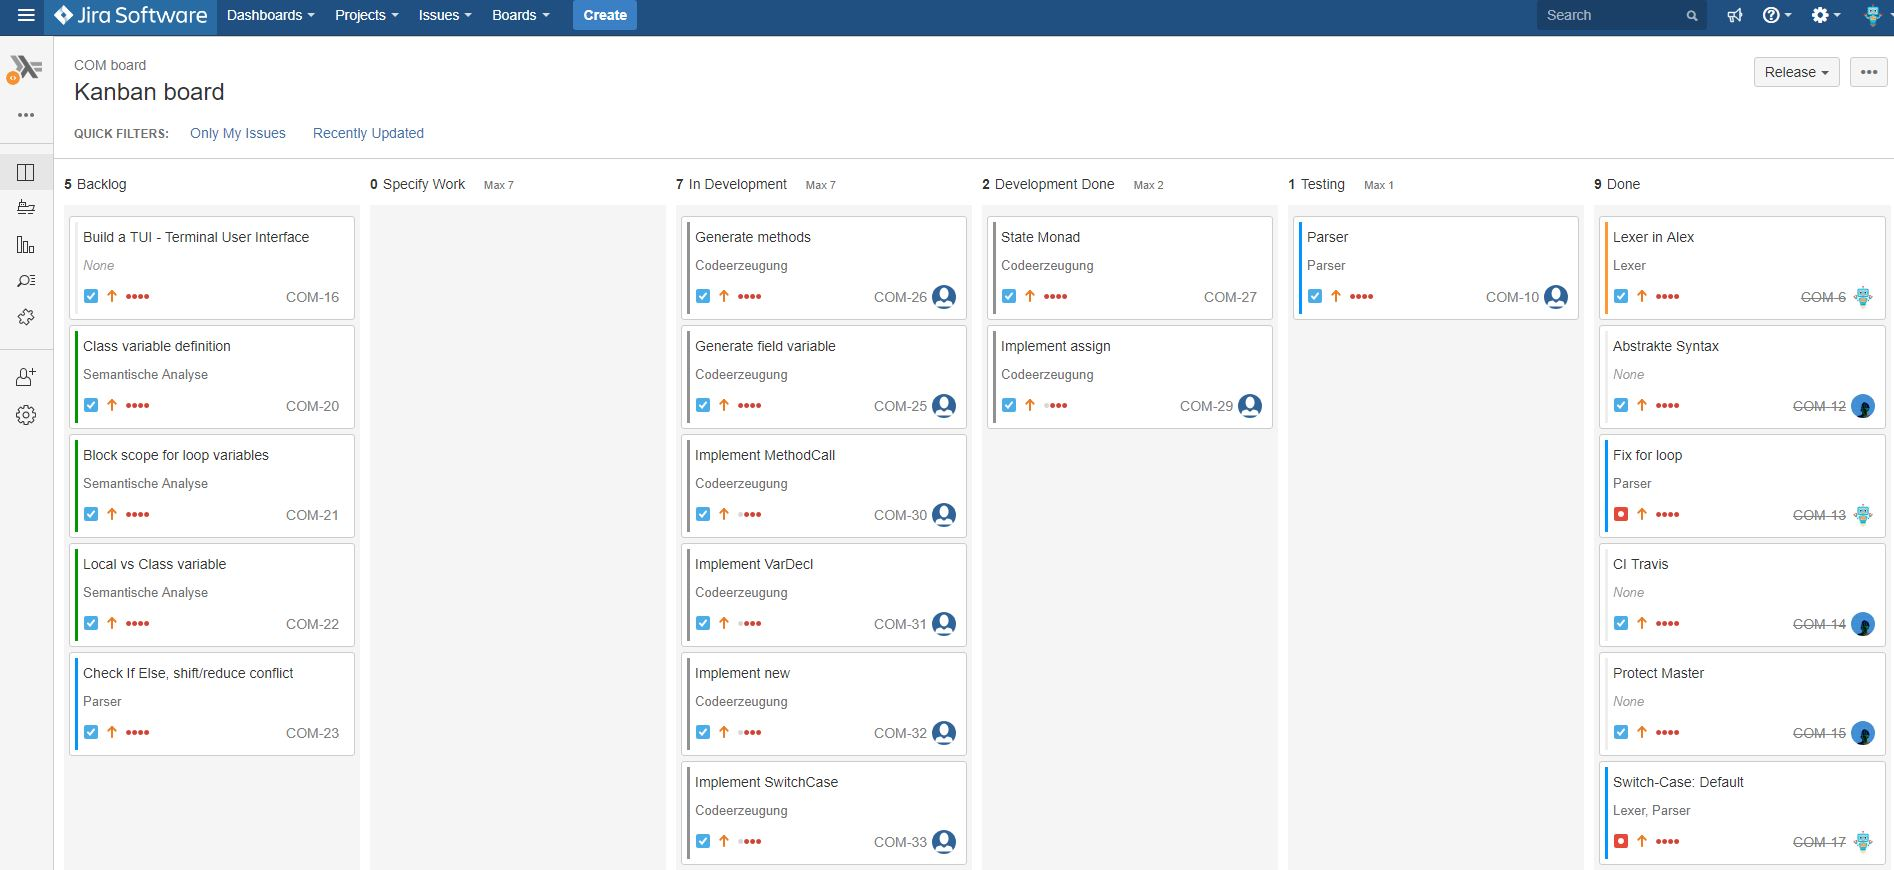
\includegraphics[scale=0.25]{images/jira.jpg}

\end{frame}


	% Struktur:
	% Allgemein
	% Abstrakte Syntax
	%  - Bsp. zeigen
	%  - Wie sind Typen abgebildet
	% Test framework
	%  - Aufbau des Frameworks
	%  - Bsp. ein Testfall etc.
	% Parser
	%  - Lexer aufbau
	%  - Happy File
	%  - Beispiel klasse
	% Typchecker
	%  - ...
	% Codegenerierer
	%  - ...
	% Abschließendes Beispiel

\end{document}
